\documentclass{beamer}

% config du thgeme metropolis
\usetheme[progressbar=frametitle,block=fill, titleformat=smallcaps,sectionpage=progressbar,]{metropolis}



\title{Analyse en Composantes Principales}
\subtitle{}
\date{2021-2022}
\author{Paul Chapron \& Yann Ménéroux}
\institute{IGN-ENSG-UGE}



%definition de la couleur du texte dans la balise \alert{}
\definecolor{vertIGN}{HTML}{96C31E} % vert IGN
\setbeamercolor{alerted text}{fg=vertIGN}



% code pour placer le log ENSG dans le bandeau de titre 
\makeatletter
\setbeamertemplate{frametitle}{%
  \nointerlineskip%
  \begin{beamercolorbox}[%
      wd=\paperwidth,%
      sep=0pt,%
      leftskip=\metropolis@frametitle@padding,%
      rightskip=\metropolis@frametitle@padding,%
    ]{frametitle}%
  \metropolis@frametitlestrut@start%
  \insertframetitle%
  \nolinebreak%
  \metropolis@frametitlestrut@end%
  \hfill
  \raisebox{-0.6ex}{
\includegraphics[height=4ex,keepaspectratio]{img/logoENSG_small.jpg}}
  \end{beamercolorbox}%
}
\makeatother




% logo ENSG première page 
\titlegraphic{\vspace{4cm}\flushright
\includegraphics[width=2cm,height=2cm]{img/logoENSG_big.png}} 



\begin{document}
\metroset{background=dark} % change background theme according to manual
\maketitle	

\section{Introduction} 

\begin{frame}{Dans les cours précédents ... }


Techniques pour quantifier la liaison entre \alert{deux} variables (quali ou quanti). 

\begin{itemize}
\item corrélation
\item régression linéaire
\item $\chi^2$  (test d'indépendance)
\item visualisation adéquate 
\end{itemize}

\end{frame}


\begin{frame}{Motivation}


La plupart des phénomènes intéressants (sociaux, spatiaux) sont \alert{multi-factoriels}. Les données disponibles pour les décrire sont :

\begin{itemize}
	\item partiellement \alert{redondantes}  :   e.g. revenu et profession
	\item intrinsèquement \alert{corrélées} : e.g. revenu et taille du logement
	\item parfois des proportions (somme à 1 ou 100\%)
\end{itemize}
\end{frame}

\begin{frame}{Quoi et Comment}
L'analyse \alert{factorielle}  cherche à réduire la \alert{colinéarité} et le \alert{nombre de dimensions} (=variables) qui décrivent une population ... 

\medskip \medskip

... en proposant de nouvelles variables \alert{composites décorrélées}.
\end{frame}


\begin{frame}{Une population}
\centering
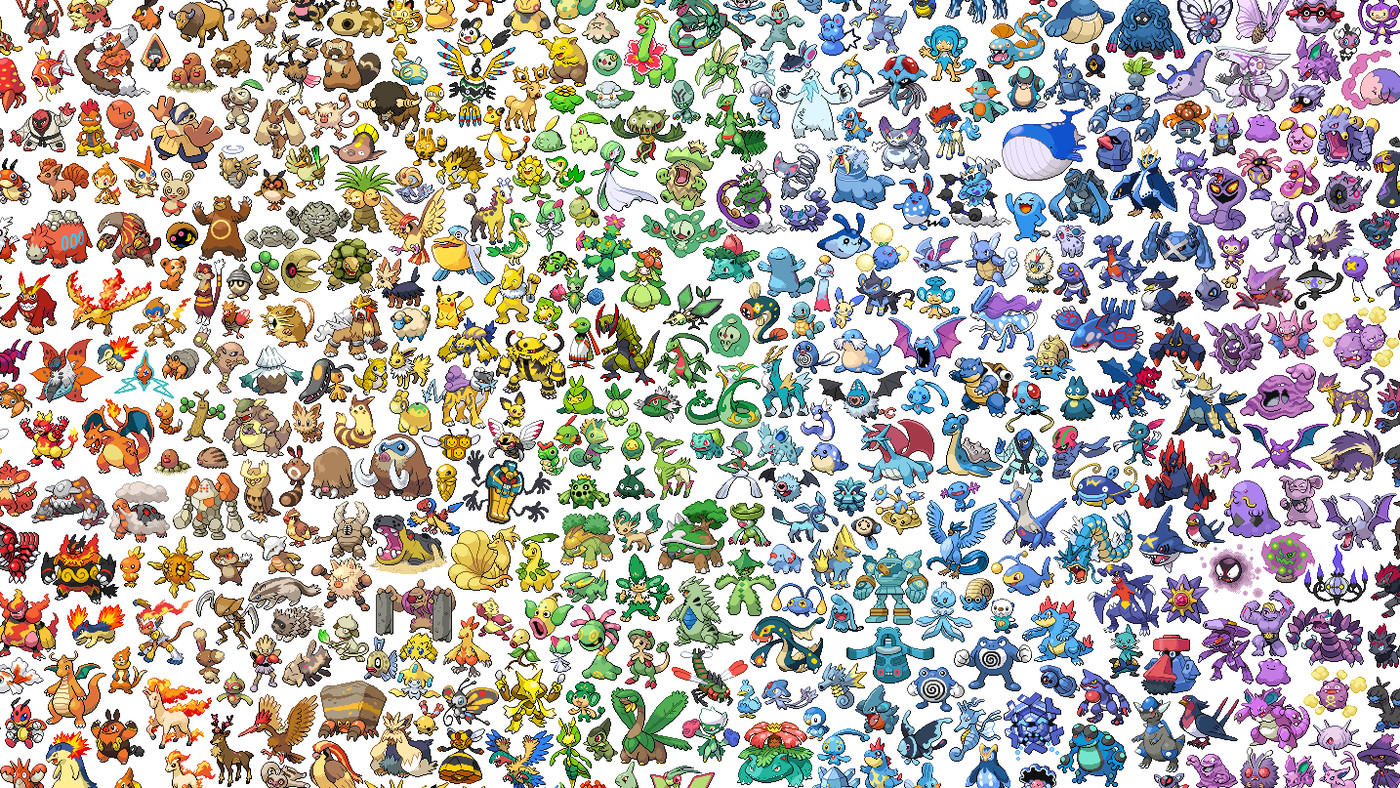
\includegraphics[width=\textwidth,keepaspectratio]{img/pokemons.jpeg}
\end{frame}

\begin{frame}{Plusieurs dimensions}
\centering
\begin{itemize}
	\item Nom e.g. "Pikachu"
	\item Type 1 $\in\{Grass,\ Fire,\ Water,\ Bug, \dots \}$
	\item Type 2 idem
	\item HP : numérique 
	\item Attack : numérique 
	\item Defense : numérique 
	\item Speed : numérique 
	\item Special Attack :numérique 
	\item Special Defense  : numérique
	\item Generation : facteur $\in \{1,2,3,4,5,6\}$
	\item Legendary : booléen
\end{itemize}

\end{frame}


\begin{frame}{Dimensions "composites"}


Existe-t-il des combinaisons  qui résument bien les caractéristiques des pokemons ? (Moins de six!)

\medskip \medskip

Comment les constituer ? 

\medskip \medskip

i.e. comment combiner les six variables numériques pour bien expliquer leur variation au sein de la population ? 



\end{frame}

\begin{frame}{Attack vs. Defense}
\centering
\includegraphics[width=\textwidth,keepaspectratio]{img/Attack_Defense.png}
\end{frame}


\begin{frame}{Speed vs. HP}
\centering
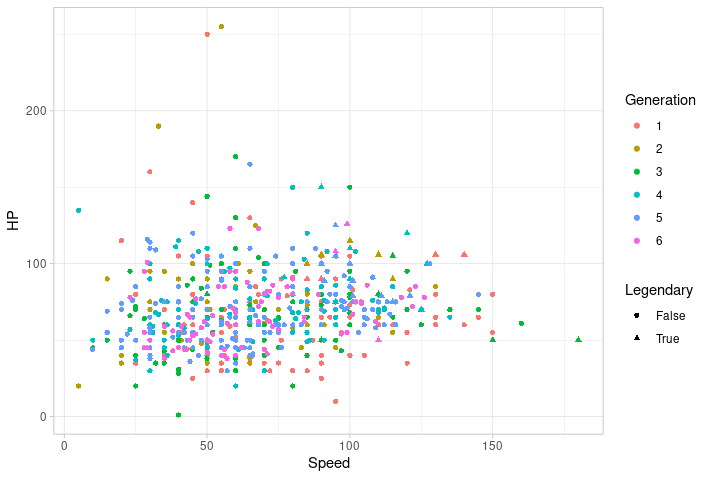
\includegraphics[width=\textwidth,keepaspectratio]{img/Speed_HP.png}
\end{frame}




\section{L'inertie}


\begin{frame}{L'inertie}
L'inertie est l'équivalent \alert{multi-dimensionnel} de la \alert{variance} d'une variable.


C'est une notion centrale de l'ACP.


$$I= \frac{1}{n}\sum_{i=1}^n d(x_i,g)$$

Avec 
\begin{itemize}
\item $n$ la taille de la population 
\item $x_i$ la valeur de la variable de l'individu $i$ 
\item $g$ le point moyen 
\item $d(x,y)$ une distance, souvent euclidienne : $(x_i-g_i)^2$ 
\end{itemize}
\end{frame}


\begin{frame}{L'inertie}


L'inertie quantifie la \alert{dispersion} du nuage de points

C'est la \alert{somme des variances} des variables

Inertie faible $\implies$ peu de variété dans les variables, individus semblables, faible quantité d'information
\end{frame}


\begin{frame}{L'inertie en 1D}


Soit une population $P$ de $n$ individus décrits par une variable $X$

l'inertie de la population est la \alert{variance} de $X$ : 

$$I= \frac{1}{n}\sum_{i=1}^n (x_i-\bar{x})^2$$

Le point moyen a pour "coordonnées" $\bar{x}$

\end{frame}


\begin{frame}{L'inertie en 2D}


Soient $X$ et $Y$ deux variables qui décrivent des individus $p_i$ de la population $P$, et $g=(x_g,y_g)$ le point (individu)  moyen de cette population de coordonnées $\bar{x}$ et $\bar{y}$.


L'inertie de $P$ est :  $$I= \frac{1}{n}\sum_{i=1}^n (x_i-x_g)^2 + (y_i-y_g)^2$$

On reconnaît une somme de variances : $I=var(X)+var(Y)$

\end{frame}


\begin{frame}{L'inertie en nD}

Soient  $v$ variables , notées $X^{(k)}, k \in \{1,\dots,v\}$ qui décrivent les individus d'une population $P$, le point moyen de $P$ est noté $g$.

L'inertie de $P$ est :  $$I= \frac{1}{n}\sum_{k=1}^v\sum_{i=1}^n (x_i^{(k)}-x^{(k)}_g)^2$$

on reconnaît $$I= \sum_{k=1}^v var(X^{(k)})$$

\end{frame}



\section{Espaces, vecteurs, axes, variables}


\begin{frame}{Individus dans l'espace d'origine}
L'ACP considère une population statistique décrite par plusieurs variables continues.


Ces variables définissent un \alert{espace vectoriel} , qu'on va appeler l'espace d'\alert{origine}: 
\begin{itemize}
	\item un individu $i$ est un \alert{vecteur}
	\item la valeur de ses variables sont les \alert{coordonnées} du vecteur dans cet espace. 
	\item chaque variable est une \alert{dimension} de cet espace. elle définit un \alert{axe} de l'espace. (cf. axe des $x$ dans un repère orthonormé)
\end{itemize}

Les variables étant potentiellement \alert{corrélées}, les axes ne sont pas toujours orthogonaux ! 

\end{frame}



\begin{frame}{Explicitation de l'ACP}


L'ACP consiste à trouver de  \alert{nouveaux axes orthogonaux entre eux}, qui capturent le \alert{plus d'inertie possible} de la population $P$.


On trouve ces axes en combinant (linéairement), les variables de la population $P$ : e.g. 

$$ axe = \alpha X + \beta Y + \gamma Z $$ 

L'algèbre linéaire nous donne la composition de ces combinaisons (les valeurs de $\alpha, \beta, \gamma$) pour chaque des nouveaux axes
\end{frame}



\begin{frame}{Exemple en 2D}



\end{frame}


\begin{frame}
TODO SCHEMA


espace de départ -> ACP -> espace d'arrivée 

\end{frame}




\begin{frame}{Calcul des axes}

Les \alert{axes} sont les \alert{vecteurs propres} de la matrice de corrélation de $P$. 
On peut les calculer ! (ouf)

\medskip

l'ACP est le calcul d’une transformation linéaire qui \alert{re-projette} des vecteurs-individus dans un nouvel \alert{espace} -- l'espace d'arrivée--  constitué par les \alert{nouveaux axes}.

\medskip

En général on choisit $\#axes < \#dimensions$ pour \alert{réduire la dimensionnalité} 


On appelle ces axes \alert{composantes}, elles sont \alert{linéairement indépendantes} et forment une \alert{base} de l'espace d'arrivée.
\end{frame}



\begin{frame}{Nombres de composantes et inertie}



\end{frame}




\begin{frame}{Nombres de composantes et inertie}


Gavish \& Donoho (2014) present a long overdue result on this problem and their answer is surprisingly simple and concrete. Essentially, the optimal procedure boils down to estimating the noise in the dataset, $\sigma$ , and then throwing away all components whose singular values are below a specified threshold. For a square $n \times n$  matrix, this threshold is:

$$\lambda = \frac{4 \sigma \sqrt{n}}{\sqrt{3}}$$


\end{frame}


\begin{frame}{L'espace d'arrivée}

On sait passer de l'espace de départ à l'espace d'arrivée : 
On peut \alert{projeter} les variables et les individus dans l'espace d'arrivée

\medskip

De cette projection on tire beaucoup d'information utiles: 


\begin{itemize}
\item regroupements d'individus
\item corrélations de variables
\item contribution / représentation  des variables 
\item contribution / représentation des individus 
\end{itemize}
\end{frame}








\begin{frame}{L'espace d'arrivée}

Contributions/ représentation  des variables 

Contribution / représentation des individus 

\end{frame}








\begin{frame}{Bilan de l'ACP}


  \begin{columns}[T,onlytextwidth]
    \column{0.5\textwidth}
        \begin{alertblock}{Avantages}
        	\begin{itemize}
        		\item Réduit la dimensionnalité
        		\item Regroupe les variables et les individus 
        	\end{itemize}
      	\end{alertblock}

    \column{0.5\textwidth}
	\metroset{block=fill}
    
      \begin{block}{Limites}
        Composantes difficiles à interpréter en elles-mêmes
      \end{block}

      
  \end{columns}
\end{frame}




\begin{frame}
\end{frame}




\begin{frame}{Animation}
  \begin{itemize}[<+- | alert@+>]
    \item \alert<4>{This is\only<4>{ really} important}
    \item Now this
    \item And now this
  \end{itemize}
\end{frame}



\begin{frame}[standout]
Mono message sur une diapo
\end{frame}


\begin{frame}{Formules}
  \begin{equation*}
    A = \sum_{i=1}^{n} \left(1 + \frac{1}{x_i}\right)^{\alpha}
  \end{equation*}
\end{frame}


\end{document}